%%%%%%%%%%%%%%%%%%%%%%%%%%%%%%
% 	   美赛模板,正文部分		 %
%          PAPER.tex         %
%%%%%%%%%%%%%%%%%%%%%%%%%%%%%%

\documentclass[12pt]{article}

% 请在此填写控制号、题号和标题
% 年份不需要填(自动以当前电脑时间年份为准)
\usepackage[]{easymcm}\problem{}
\usepackage{palatino} % 这个是COMAP官方杂志的字体,如不需要可注释掉,以使用默认字体
\usepackage{graphicx}
\graphicspath{{figures/}}
\usepackage{amsmath}
\usepackage{lscape}
\usepackage{CJK}

\title{}  % 标题

% 正文开始
\begin{document}
%%%%%%%%%%%%%%%%%%%%%%%%%%%%%%%%%%%%%%%%%
%%            请在此填写摘要            %%
%%%%%%%%%%%%%%%%%%%%%%%%%%%%%%%%%%%%%%%%%
\begin{abstract}\small
    Here is the abstract of your paper.

    Firstly, that is ...

    Secondly, that is ...

    Finally, that is ...

\end{abstract}



%%%%%%%%%%%%%%%%%%%%%%%%%%%%%%%%%%%%%%%%%%
% 如不理解以下部分中各命令的含义,请勿修改! %
%%%%%%%%%%%%%%%%%%%%%%%%%%%%%%%%%%%%%%%%%%

%---------以下生成sheet页----------
% 下面的语句可调整全文行距为标准值的0.6倍,请自行使用
%\renewcommand{\baselinestretch}{0.6}\normalsize
%\maketitle  % 生成sheet页
\thispagestyle{empty}   % 不要页眉页脚和页码
\setcounter{page}{0} % 此命令仅是为了避免页码重复报错,不要在意

%---------以下生成目录----------
\newpage
\tableofcontents
\thispagestyle{empty}   % 不要页眉页脚和页码
\newpage

%---------以下生成正文----------
\setlength\parskip{0.8\baselineskip}  % 调整段间距
\setcounter{page}{1}    % 从正文开始计页码
\pagestyle{fancy} 		% 摘要请到ABSTRACT.tex中填写


\section{Introduction}
\subsection{Project Background Information}
Dalian is an important central city, port and tourist city in the northern coastal areas of China. Dalian is located on the east coast of Eurasia, the southernmost point of the Liaodong Peninsula in northeast China, the Yellow Sea in the east, the Bohai Sea in the west, the Shandong Peninsula across the sea in the south, and the vast northeast plain in the north. It is an important sea gateway in northern China. With the rapid development of regional social economy, the population of Dalian has been increasing. At the end of 2014, the city's registered population was about 5.943 million. The resident population was mainly concentrated in the central city and related peripheral streets, with about 4.1 million people, of which the permanent population in the core area accounted for more than 65\% of the permanent population in the central city.$^{[1]}$
\par As the growth rate of transportation demand is higher than the construction speed of transportation facilities, road resources and public transportation facilities cannot meet the travel demand, and the contradiction between supply and demand is prominent. Dalian is committed to developing public transportation to alleviate this pressure. In order to solve the current problems in Dalian's transportation, adapt to the needs of urban economic growth and development, and adapt to the sustainable development of urban transportation, the Dalian People's Government compiled and completed the “Dalian Urban Rail Transit Network Planning”. (2015-2020) and “Dalian Urban Rail Transit Construction Planning (2015-2020), (hereinafter referred to as “Construction Planning”). According to the "Construction Plan", the third phase of the Metro Line 1 , Line 4, Line 5 (hereinafter referred to as "Metro Line 5") and Phase II of the R4 Line will be built from 2015 to 2020.


\subsection{Innovation}
Metro Line 5 is the first rail transit investment project in Dalian that uses the whole process of cooperation between the government and the social capital. The social capital procurement, contract negotiation and project company registration are being completed.

\subsection{Necessity}

From a qualitative point of view, the project adopts the PPP model to increase public supply, optimize risk allocation, improve efficiency, promote management innovation and fair competition, and effectively implement government procurement policies compared with the traditional government investment and procurement model; Can also effectively alleviate the traffic pressure in Dalian
From a quantitative point of view, the value-for-value evaluation value and the value-for-money index of the project are both greater than zero, and the PPP mode is suitable.


\section{Research Project content}
\subsection{Research content}
Dalian Metro Line 5 has a total length of 24.484 kilometers. It is laid by underground line, with 18 stations (including 6 interchange stations), 1 vehicle section, 1 control center and 2 main substations. The main construction contents include stations, sections, depots, control centers and related equipment and facilities. Dalian Metro Group and the project company signed a “Franchise Agreement” to grant the project company a franchise right; the project company is responsible for the investment and financing of the project’s, construction, operation, renewal and maintenance work.
\par Metro Line 5 is connected in series with the core carrier of Qingniwa and Shuttle Fish Bay. It connects Dalian Railway Station and Dalian New Airport to two external transportation hubs. It breaks the bay against Qingniwa, the Bayu Bay area and even the old Ganjingzi. The blockage of the area has changed the single westward passage of the Ganjingzi area in the past, providing a new way of travel for the Ganjingzi area. The capacity of Dalian Express Rail Line 3 (R3) is close to saturation and is expanding. According to the current passenger flow section analysis of the fast track No. 3 line, the post-salt to the railway station is the area with the largest passenger flow pressure on the R3 line, while the subway line 5 is transferred twice at the train station and the post-salt and fast-track line 3, which can be effective. Relieve passenger flow pressure in the core area of Fast Track Line 3.
\subsection{Plan content}
According to the plan, Metro Line 5 starts from the Ocean Plaza at the intersection of Binhai East Road and Hutan Road in Hutan New District in the south, and passes through the Tiger Beach Park to the west and then to the east side of the Labor Park along the Jiefang Road in the northwest. Entering the friendly street to the north, after crossing the Harbin-Dalian Railway, go to the Dalian Railway Station North Square, cross the bay and enter the Barracuda Bay area, go north along the Ganjingzi Road to the spring water, post-salt, and wear the Shenhai Expressway. After the 202 National Highway, the terminal is located at Houguancun Station, and the new extension is connected to the north extension of Dalian Metro Line 1. The route map is showed in figure


\begin{figure}[htbp]
	\centering
	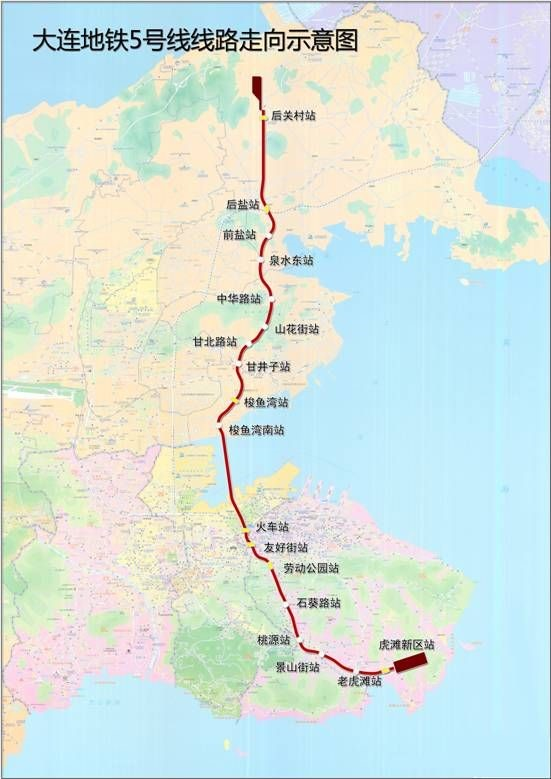
\includegraphics[width=6in]{figures/01.jpg}
	\caption{The Route Map}
%	\label{fig:2}
\end{figure}

\newpage
\section{Project economic analysis}
\subsection{Demand analysis}
The key factor for the rapid development of the urban rail market is the continuous establishment and opening of the new line. Since 2014, the demand for the urban rail market including subways, trams, and light rails has gradually been released. The major first-tier and second-tier cities have basically obtained the qualifications for urban rail construction and began to enter the stage of intensive construction period. Rail transportation helps to enrich residents' travel modes, establish an efficient, flexible and environmentally friendly urban transport system, also help to increase the price of land assets along the line and activate urban development.
Another factor is the increasement in the density of existing urban rail transit lines. This is because the substitution of urban rail for public transportation and other modes of travel is gradually increasing, and the passenger flow intensity of the line often increases with the extension of operation time.
In the early days of line operation, the number of residents who chose urban rail transportation was lower because traditional travel habits had not been reversed. With the maturity of urban rail operations and the increasing dependence of residents on the urban rail system, the passenger flow density will gradually increase.$^{[2]}$
The data shows that the passenger flow intensity is inversely related to the minimum departure interval during the peak period, and has a significant positive correlation with the distribution density. That is, the greater the operational intensity and the higher the daily average passenger flow intensity per kilometer, the higher the distribution density.

\begin{figure}[htbp]
	\centering
	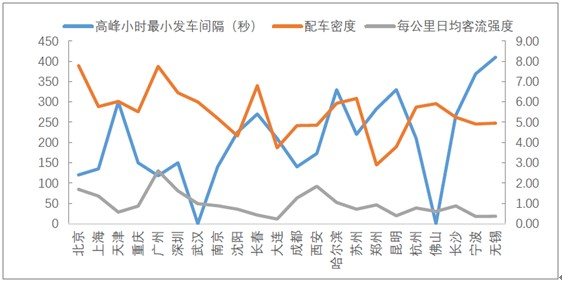
\includegraphics[width=6in]{figures/02.jpg}
	\caption{command analysis}
%	\label{fig:2}
\end{figure}



Above all, with the increasing flow of passengers, the lines need to be put into construction urgently.

\subsection{Cost analysis}
\subsubsection{Found rasing plan}
The shareholders of the limited liability company shall be responsible for the company within the limits of the capital contribution they have subscribed. Since the project is a major infrastructure project in Dalian, the investment amount is huge and the life cycle is long, which faces many unpredictable during the construction and operation of the project. Various types of risks, appropriate increase of project capital ratio is conducive to better prevention of risks; at the same time, when the project capital ratio is low, the project company has a higher financing risk, considering the reasonable profit of the project company and the bank financing cost (long-term benchmark Interest rate 4.9\%) and other domestic similar project experience data, under the premise of the internal rate of return of project capital of 8\%, the capital ratio of the project is considered at 40\% of the total investment, and the remaining 60\% of the funds are considered solving by bank loans. The loans used for construction investment and construction period interest are considered based on the long-term loan interest rate. The loan period is 24.5 years, the grace period is 5.5 years, and the repayment period is 19 years. The interest rate based on the current 5-year long-term loan annual benchmark interest rate issued by the People’s Bank of China is 4.9\%. The loan used by working capital is a short-term loan, and the interest rate is calculated based on the current one-year short-term loan annual interest rate issued by the People's Bank of China, which is 4.35\%.$^{[3]}$

\subsubsection{Total cost}
\begin{itemize}
    \item {\bfseries Power costs.} Refer to all traction, power, and lighting. Refer to the domestic subway operation data and domestic similar project data in combination with the local price level. The project is temporarily calculated according to 5.5 degrees / car kilometers (including tax), the electricity price is calculated according to the current Dalian Metro agreement electricity price of 0.695 yuan/kWh (including tax).
    \item {\bfseries Repair costs.} Include vehicle repair costs, mechanical and electrical equipment repair costs, and major repairs and daily maintenance costs for tunnels, building construction, and reference to domestic subway operating data and domestic similar project data combined with local price levels. The project is temporarily calculated at 3.5 yuan / car kilometers (including tax).
    \item {\bfseries Operating expenses.} Operating expenses refer to the expenses related to operations, including water, transportation, accident, metering, ticket printing, cleaning, etc. According to the domestic subway operation data, the project is calculated at 1.5 yuan/car km.
    \item  {\bfseries Labor Wages.} Personnel's salary is based on the feasibility study report. The initial, near and long-term quotas of the project are 56 persons/km, 59 persons/km, and 57 persons/km respectively. According to the approval of the Dalian Financial Department, the average salary of the subway operation company in 2016 was 67,600 yuan (before tax), and the welfare expenses were 40.1\% of the salary. According to this calculation, the initial period of the staff salary (including welfare) is 94,700 yuan/year[9.47 = 6.76 * (1 + 40.1\%)]
    \item  {\bfseries Management fee.} The management fee is considered as 10\% of the above sum.
    \item  {\bfseries Operating cost adjustment.} The above-mentioned operating cost adjustment is the operating cost of the project. Considering the cost increase, the estimated operating cost is increased by the annual average of 3\% inflation coefficient.

\end{itemize}




\subsection{Income analysis}

\begin{itemize}
  \item {\bfseries Ticket income} The ticket price for the Dalian Metro fare is implemented as follows: The fare standard is as follows:
  \item {\bfseries Fare adjustment} Considering the fare adjustment of the subway, the average fare of the project is adjusted every five years according to the annual average 2\% fare growth rate.
  \item {\bfseries Non-ticket revenue}  Non-ticket revenue is estimated at 20\% of the ticket revenue.
  \item {\bfseries Subsidy income (Also calculate tax)} The subsidy income is divided into two parts: First, the annual construction cost subsidy, that is, the construction cost subsidy paid by the government in each year of the operation period, including the total construction investment (including other construction costs, construction period interest), operating period interest, taxes and fees. Reasonable return (annual construction cost subsidy is PPP trademark, that is, social capital quote)
The second is the operational feasibility gap subsidy (fare compensation), which is the passenger difference between the agreed per capita fare (PPP bidding, the quoted social capital) and the predicted per capita fare.
  \item {\bfseries Turnover tax and surcharge} Urban maintenance and construction tax: According to national regulations, it is calculated as 7\% of value-added tax.
 Education surcharge: According to national regulations, it is 3\% of value-added tax.
 Local education surcharge: According to national regulations, 2\% of the value-added tax.
 The above four taxes are listed in the VAT and additional items.
\end{itemize}






\section{Financial Analysis}
\subsection{Investment Analysis}

In table \textbf{Table \ref{tb:notation}}.Notations will be used are defined.
\begin{table}[!htbp]
\begin{center}
\caption{Notations}
\begin{tabular}{cl}
	\toprule
	\multicolumn{1}{m{3cm}}{\centering Symbol}
	&\multicolumn{1}{m{8cm}}{\centering Definition}\\
	\midrule
	$k$&Serial\,\,Number\,\,of Subproject Investment\\
    $n$&Serial\,\,Number\,\,of Project Investment\\
    $m$&Serial\,\,Number\,\,of Part Investment\\
    $y$&Year\,\,Number\\
	$SPI_k$&Subproject\,\,Investment\,\,of k Subproject\\
    $PPI_n$ &Project\,\,Investment\,\,of n Project\\
    $PI_m$ &Part\,\,Investment\,\,of m Part\\
	$TI$ &Total\,\,Investment\\
    $IFIR$ &Inflection-free\,\,Interest\,\,Rate\\
    $IR$ &Inflaction\,\,Rate\\
    $MR$ & Market Rate\\
    $PTI_{2016}$&\text{2016 }Present\,\,Total\,\,Interestment\,\,\\
    $PTI_{2021}$&\text{2021 }Present\,\,Total\,\,Interestment\,\,\\
    $AWC$ &Additional Working Capita\\
    $AMWC$ &Amount of Working Capital\\
    $IRR$ &Internal Rate of Return\\
    $PW$ &Present Value\\
	\bottomrule
\end{tabular}\label{tb:notation}
\end{center}
\end{table}


We first collected the detail data of the project, it is composed by four parts I, II, III and IV. Each part is composed by some projects and some of these subjects are composed by sub-projects. For example, in part I, the investment of project 1 is the sum of subproject 1.1, 1.2 and 1.3.
\begin{itemize}
  \item {\bfseries 1.} Use formula (1) to calculate $PPI_n$:
        \begin{equation}\label{1}
            PPI_n=\varSigma SPI_k
        \end{equation}
  \item {\bfseries 2.} Use formula (2) to calculate $PI_m$:
        \begin{equation}\label{2}
            PI_m=\varSigma PPI_n
        \end{equation}
  \item {\bfseries 3.} Use formula (3) to calculate the year $y$ 's total investment $TI_y$:
        \begin{equation}\label{3}
            TI_y=\varSigma PI_m
        \end{equation}
  \item {\bfseries 4.} Use {\bfseries Present Value Analysis} to find the Present Value of 2016 $PTI_{2016}$, which is composed by the {\bfseries initial present value} and {\bfseries calculated present value} $PTI_{2016}$.The $Excel$ function $NPV$ is used to calculate $Present Worse$ in 2016 it can be treated as {\bfseries calculated present value}:
        \begin{equation}\label{4}
         PTI_{2016}=NPV\left( MR,\left[ SI_k \right] \right) +PTI_{2016}
         \end{equation}
  \item {\bfseries 5.} Use formula(5) to calculate $MR$:
        \begin{equation}\label{5}
          MR=IFIR+IR+IFIR\times IR
        \end{equation}
  \item {\bfseries 6.} The investment $PTI_{2021}$ is based on $PTI_{2016}$ is affected by $MR$, $PTI_{2021}$ use formula(6) to calculate $PTI_{2021}$:
        \begin{equation}\label{6}
          PTI_{2021}=PTI_{2016}\times \left( 1+MR \right) ^5
        \end{equation}
\end{itemize}

\subsection{Cash Flow Statement Analysis}
Cash Flow Statement consists of three parts which are Operating Activities, Investment Activities and Financing Activities.

\par {\bfseries 1. In Operating Activities} There are net income and depreciation. Both these two items are calculated in Income Statement Table.
\par {\bfseries 2. In Investment Activities}  There are investment of equipment and infrastructure, Salvage Value, Gain Taxes and Working capital.
\par Investment of {\bfseries Equipment and Infrastructure} is estimated in the Project Investment Table. The investment form 2016 to 2021 is converted to the investment in 2021. The the total investment of equipment and infrastructure is $2,105,264$ according to the calculating result in the Project Investment Table. Since the investment is the cash outflow, it is $-2,105,265$.
\par {\bfseries Salvage Value} is estimated according to the types and number of equipment. Since the salvage value is the residual value that expected to be recovered when an asset expires, it is $700,000$ at the inflation rate of $\%3.74$.
\par $Gain Taxes$ is related to depreciation and salvage value. The formula is as formula(7)
\begin{equation}\label{}
  Gains\,\,Taxes=\left( Slavage\,\,Value-Book\,\,Value_n \right) *\left( Tax\,\,Rate \right)
\end{equation}
In which book value is:
\begin{equation}\label{}
  BookVlaue=BasisCost-\sum{Depreciation}
\end{equation}

In which Tax Rate is the same as the tax rate in the Income Statement Table, which is $33\%$. In $Excel$ The Book Value is calculated according to the Depreciation Table. The function is
\begin{equation}\label{}
  BookValue=1746548-(SUM(D1,D2,\ldots,D10))=1746548-1068020=678528
\end{equation}
And the Gains taxes is
\begin{equation}\label{}
  GainsTaxes=(700000-678528)*0.33=7086
\end{equation}

{\bfseries Working capital} is the amount money available for the daily use and turnover in the operation of rail transportation. It’s estimated according to other transportation project with the same scale. The working capital of 2021 is -45,000. Taken the inflation rate of $3.74\%$ into consideration, the additional working capita($AWC$) of each following year is calculated as follows:
\begin{equation}
  {AWC}_{2022}=-45000\ast3.74\%=-1683
\end{equation}
\begin{equation}\label{}
   {AWC}_{i+1}={AWC}_i\ast(1+3.74\%)
\end{equation}
\begin{equation}\label{}
  {AWC}_{2023}={AWC}_{2022}\ast1+3.74\%=-1683*1+3.74\%=-1,746
\end{equation}
$$\ldots$$
\begin{equation}\label{}
  {AWC}_{2030}={AWC}_{2029}\ast(1+3.74\%)=-2,176\ast(1+3.74\%)=-2,258
\end{equation}
As this project is a 10-year project, it needs to retrieve all the working capital in the end of 10th year. Therefore, the amount of working capital($AMWC$) this project invested is
\begin{equation}\label{}
  AMWC=\sum_{i=2021}^{2030}{-AWC_i}
\end{equation}

\par {\bfseries 3. Financing Activities}, there are borrowed funds and principle repayment.{\bfseries Borrowed Funds }is $660,688$ in 2021 according to the Loan Repayment Table.{\bfseries Principle Repayment} is also calculated in the Loan Repayment Table.
\par {\bfseries 4. Net Cash Flow} of each year is the sum of the items above of that year.
\par {\bfseries 5. Internal Rate of Return $(IRR)$} is the interest rate when the present value equals to zero, which means the amount of cash inflow is equal to outflow. Use the fomula in Excel:
\begin{equation}\label{}
  IRR(values, guess rate)
\end{equation}
The $IRR$ can be calculated as $-1\%$.Because we assume the project period is only 10 years. However, the project life can be 20 years or even more. Consider the $IRR$ of more than 10 years, it may be positive.
\par {\bfseries 6. Present Value} based on the current interest rate, use the formula as following:
\begin{equation}\label{}
  PW=NPV({MarketInterestRate,CashFlow}_{1,2,\ldots,n})+{CashFlow}_0
\end{equation}
In which current Market Interest rate is $8.823\%$ according to the Project Investment Table.$PW$ is calculated as $-770567$.



\begin{table}[htbp]
\small
  \centering
  \caption{Total Project Investment Analysis}
    \begin{tabular}{l|l|l|l|l|l|l|l}
    \multicolumn{8}{|p{22.28em}}{\textbf{Total Project Investment}} \\
    \multicolumn{8}{l}{\textbf{(Unit: 10,000 yuan¥)}} \\
    \rowcolor[rgb]{ .929,  .49,  .192} \multicolumn{1}{p{1em}|}{\textcolor[rgb]{ 1,  1,  1}{\textbf{k}}} & \multicolumn{1}{c|}{\textcolor[rgb]{ 1,  1,  1}{\textbf{Name}}} & \textcolor[rgb]{ 1,  1,  1}{\textbf{2016}} & \textcolor[rgb]{ 1,  1,  1}{\textbf{2017}} & \textcolor[rgb]{ 1,  1,  1}{\textbf{2018}} & \textcolor[rgb]{ 1,  1,  1}{\textbf{2019}} & \textcolor[rgb]{ 1,  1,  1}{\textbf{2020}} & \textcolor[rgb]{ 1,  1,  1}{\textbf{2021}} \\
    \hline
    \rowcolor[rgb]{ .973,  .796,  .678} \textbf{I} & \textbf{Project costs} &      53,427  &    186,913  &             221,360  &    259,021  &    273,198  &    186,577  \\
    \hline
    \rowcolor[rgb]{ .988,  .894,  .839} \textbf{1} & \textbf{Station engineering} &      26,028  &      55,687  &               55,687  &      63,677  &      53,629  &      47,940  \\
    \hline
    \rowcolor[rgb]{ .973,  .796,  .678} \textbf{1.1} & \textbf{Construction } &        1,816  &        7,264  &                 7,264  &        7,264  &        9,079  &        3,632  \\
    \hline
    \rowcolor[rgb]{ .988,  .894,  .839} \textbf{1.2} & \textbf{Equipment} &       &       &       &        7,990  &        8,232  &        7,990  \\
    \hline
    \rowcolor[rgb]{ .973,  .796,  .678} \textbf{1.3} & \textbf{structure} &      24,212  &      48,424  &               48,424  &      48,424  &      36,318  &      36,318  \\
    \hline
    \rowcolor[rgb]{ .988,  .894,  .839} \textbf{2} & \textbf{District engineering} &      18,690  &      74,762  &               74,762  &      74,762  &      74,762  &      56,071  \\
    \hline
    \rowcolor[rgb]{ .973,  .796,  .678} \textbf{3} & \textbf{Track engineering} &        2,518  &      10,070  &               10,070  &      10,070  &      10,070  &        7,553  \\
    \hline
    \rowcolor[rgb]{ .988,  .894,  .839} \textbf{4} & \textbf{Wanted system} &       &        3,757  &                 7,514  &        9,392  &      13,149  &        3,757  \\
    \hline
    \rowcolor[rgb]{ .973,  .796,  .678} \textbf{5} & \textbf{Nickname system} &       &        3,398  &                 6,796  &        8,495  &      11,893  &        3,398  \\
    \hline
    \rowcolor[rgb]{ .988,  .894,  .839} \textbf{6} & \textbf{Power supply system} &       &      13,541  &               27,082  &      33,853  &      47,394  &      13,541  \\
    \hline
    \rowcolor[rgb]{ .973,  .796,  .678} \textbf{7} & \textbf{Practice and control} &       &           697  &                 1,395  &        1,744  &        2,441  &           697  \\
    \hline
    \rowcolor[rgb]{ .988,  .894,  .839} \textbf{8} & \textbf{Prevention alarm} &       &        1,733  &                 3,466  &        4,333  &        6,066  &        1,733  \\
    \hline
    \rowcolor[rgb]{ .973,  .796,  .678} \textbf{9} & \textbf{Security control} &       &           689  &                 1,378  &        1,723  &        2,412  &           689  \\
    \hline
    \rowcolor[rgb]{ .988,  .894,  .839} \textbf{10} & \textbf{Ventilation} &       &        1,991  &                 3,982  &        4,978  &        6,969  &        1,991  \\
    \hline
    \rowcolor[rgb]{ .973,  .796,  .678} \textbf{11} & \textbf{Water supply} &       &        1,502  &                 3,005  &        3,756  &        5,258  &        1,502  \\
    \hline
    \rowcolor[rgb]{ .988,  .894,  .839} \textbf{12} & \textbf{Sales inspection} &       &       &       &       &       &      13,759  \\
    \hline
    \rowcolor[rgb]{ .973,  .796,  .678} \textbf{13} & \textbf{Station attached equip} &       &       &       &      10,987  &      10,987  &      11,320  \\
    \hline
    \rowcolor[rgb]{ .988,  .894,  .839} \textbf{14} & \textbf{Control center} &        1,135  &        3,405  &                 5,999  &        6,486  &        7,945  &        7,459  \\
    \hline
    \rowcolor[rgb]{ .973,  .796,  .678} \textbf{14} & \textbf{Construction } &           195  &           584  &                    778  &           778  &           778  &           778  \\
    \hline
    \rowcolor[rgb]{ .988,  .894,  .839} \textbf{14} & \textbf{Quality equipment} &       &       &                    389  &           519  &           908  &           778  \\
    \hline
    \rowcolor[rgb]{ .973,  .796,  .678} \textbf{14} & \textbf{Electrical Equipment} &       &       &                 1,070  &        1,427  &        2,497  &        2,140  \\
    \hline
    \rowcolor[rgb]{ .988,  .894,  .839} \textbf{14} & \textbf{structure} &           940  &        2,821  &                 3,762  &        3,762  &        3,762  &        3,762  \\
    \hline
    \rowcolor[rgb]{ .973,  .796,  .678} \textbf{15} & \textbf{Depot \& practice base} &        4,544  &      13,631  &               18,175  &      22,719  &      18,175  &      13,631  \\
    \hline
    \rowcolor[rgb]{ .988,  .894,  .839} \textbf{15} & \textbf{Special vehicles} &           727  &        2,181  &                 2,908  &        3,635  &        2,908  &        2,181  \\
    \hline
    \rowcolor[rgb]{ .973,  .796,  .678} \textbf{15} & \textbf{structure} &        3,817  &      11,450  &               15,267  &      19,084  &      15,267  &      11,450  \\
    \hline
    \rowcolor[rgb]{ .988,  .894,  .839} \textbf{16} & \textbf{Civil air defense} &           512  &        2,048  &                 2,048  &        2,048  &        2,048  &        1,536  \\
    \hline
    \rowcolor[rgb]{ .973,  .796,  .678} \textbf{II} & \textbf{Other costs} &    142,681  &      28,536  &               28,536  &      28,536  &      28,536  &      28,536  \\
    \hline
    \rowcolor[rgb]{ .988,  .894,  .839} \textbf{III} & \textbf{Reserve fee} &      19,611  &      21,545  &               24,990  &      28,756  &      30,173  &      21,511  \\
    \hline
    \rowcolor[rgb]{ .973,  .796,  .678} \textbf{IV} & \textbf{Vehicle purchase fee} &       &       &       &       &       &    117,000  \\
    \hline
    \rowcolor[rgb]{ .988,  .894,  .839}       & \textbf{Number of vehicles } &       &       &       &       &       &  \\
    \hline
    \rowcolor[rgb]{ .973,  .796,  .678}       & \textbf{Unit price} &       &       &       &       &       &  \\
    \hline
    \rowcolor[rgb]{ .988,  .894,  .839}       & \textbf{Construction Invest.} &    215,719  &    236,992  &             274,885  &    316,315  &    331,907  &    353,624  \\
    \hline
    \rowcolor[rgb]{ .973,  .796,  .678}       & \textbf{ IR=3.74\% } &       &       &       &       &       &  \\
    \hline
    \rowcolor[rgb]{ .988,  .894,  .839}       & \textbf{ IFIR=4.9\% } &       &       &       &       &       &  \\
    \hline
    \rowcolor[rgb]{ .973,  .796,  .678}       & \textbf{MIR=8.82326\%} &       &       & 8.82326\% &       &       &  \\
    \hline
    \rowcolor[rgb]{ .988,  .894,  .839}       & \textbf{2016-Present Value} &       &       &       1,379,424.8  &       &       &  \\
    \hline
    \rowcolor[rgb]{ .973,  .796,  .678}       & \textbf{2021-Present Vlaue} &       &       & \textcolor[rgb]{ 1,  0,  0}{\textbf{   2,105,264.6 }} &       &       &  \\
    \end{tabular}%
  \label{tab:addlabel}%
\end{table}%
%================

\begin{landscape}
\begin{table}[htbp]
\footnotesize
  \centering
  \caption{Cash Flow}
    \begin{tabular}{lccllllllllll}
    \hline
    \multicolumn{10}{|c|}{\textbf{Cash Flow  Statement }} \\
    \hline
    \rowcolor[rgb]{ .329,  .655,  .22} \multicolumn{1}{|l|}{\textcolor[rgb]{ 1,  1,  1}{\textbf{End of year}}} & \multicolumn{1}{l|}{\textcolor[rgb]{ 1,  1,  1}{\textbf{IR}}} & \multicolumn{1}{c|}{\textcolor[rgb]{ 1,  1,  1}{\textbf{2021}}} & \multicolumn{1}{c|}{\textcolor[rgb]{ 1,  1,  1}{\textbf{2022}}} & \multicolumn{1}{c|}{\textcolor[rgb]{ 1,  1,  1}{\textbf{2023}}} & \multicolumn{1}{c|}{\textcolor[rgb]{ 1,  1,  1}{\textbf{2024}}} & \multicolumn{1}{c|}{\textcolor[rgb]{ 1,  1,  1}{\textbf{2025}}} & \multicolumn{1}{c|}{\textcolor[rgb]{ 1,  1,  1}{\textbf{2026}}} & \multicolumn{1}{c|}{\textcolor[rgb]{ 1,  1,  1}{\textbf{2027}}} & \multicolumn{1}{c|}{\textcolor[rgb]{ 1,  1,  1}{\textbf{2028}}} & \multicolumn{1}{c|}{\textcolor[rgb]{ 1,  1,  1}{\textbf{2029}}} & \multicolumn{1}{c|}{\textcolor[rgb]{ 1,  1,  1}{\textbf{2030}}} & \multicolumn{1}{c|}{\textcolor[rgb]{ 1,  1,  1}{\textbf{2031}}} \\
    \hline
    \rowcolor[rgb]{ .784,  .886,  .984} \multicolumn{1}{|l|}{\textbf{Operating Act.}} & \multicolumn{1}{l|}{\cellcolor[rgb]{ .769,  .937,  1}} & \multicolumn{1}{l|}{\cellcolor[rgb]{ .769,  .937,  1}} & \multicolumn{1}{l|}{\cellcolor[rgb]{ .769,  .937,  1}} & \multicolumn{1}{l|}{\cellcolor[rgb]{ .769,  .937,  1}} & \multicolumn{1}{l|}{\cellcolor[rgb]{ .769,  .937,  1}} & \multicolumn{1}{l|}{\cellcolor[rgb]{ .769,  .937,  1}} & \multicolumn{1}{l|}{\cellcolor[rgb]{ .769,  .937,  1}} & \multicolumn{1}{l|}{\cellcolor[rgb]{ .769,  .937,  1}} & \multicolumn{1}{l|}{\cellcolor[rgb]{ .769,  .937,  1}} & \multicolumn{1}{l|}{\cellcolor[rgb]{ .769,  .937,  1}} & \multicolumn{1}{l|}{\cellcolor[rgb]{ .769,  .937,  1}} & \multicolumn{1}{l|}{\cellcolor[rgb]{ .769,  .937,  1}} \\
    \hline
    \rowcolor[rgb]{ .784,  .886,  .984} \multicolumn{1}{|r|}{\textit{\textbf{              Net income}}} & \multicolumn{1}{l|}{\cellcolor[rgb]{ .769,  .937,  1}} & \multicolumn{1}{l|}{\cellcolor[rgb]{ .769,  .937,  1}} & \multicolumn{1}{l|}{\cellcolor[rgb]{ .769,  .937,  1}\textbf{33,552 }} & \multicolumn{1}{l|}{\cellcolor[rgb]{ .769,  .937,  1}\textcolor[rgb]{ 1,  0,  0}{\textbf{-25,370 }}} & \multicolumn{1}{l|}{\cellcolor[rgb]{ .769,  .937,  1}\textcolor[rgb]{ 1,  0,  0}{\textbf{-5,516 }}} & \multicolumn{1}{l|}{\cellcolor[rgb]{ .769,  .937,  1}\textbf{8,748 }} & \multicolumn{1}{l|}{\cellcolor[rgb]{ .769,  .937,  1}\textbf{23,106 }} & \multicolumn{1}{l|}{\cellcolor[rgb]{ .769,  .937,  1}\textbf{34,088 }} & \multicolumn{1}{l|}{\cellcolor[rgb]{ .769,  .937,  1}\textbf{44,436 }} & \multicolumn{1}{l|}{\cellcolor[rgb]{ .769,  .937,  1}\textbf{52,644 }} & \multicolumn{1}{l|}{\cellcolor[rgb]{ .769,  .937,  1}\textbf{62,405 }} & \multicolumn{1}{l|}{\cellcolor[rgb]{ .769,  .937,  1}\textbf{100,231 }} \\
    \hline
    \rowcolor[rgb]{ .784,  .886,  .984} \multicolumn{1}{|r|}{\textit{\textbf{              Depreciation}}} & \multicolumn{1}{l|}{\cellcolor[rgb]{ .769,  .937,  1}} & \multicolumn{1}{l|}{\cellcolor[rgb]{ .769,  .937,  1}} & \multicolumn{1}{l|}{\cellcolor[rgb]{ .769,  .937,  1}\textbf{87,327 }} & \multicolumn{1}{l|}{\cellcolor[rgb]{ .769,  .937,  1}\textbf{165,922 }} & \multicolumn{1}{l|}{\cellcolor[rgb]{ .769,  .937,  1}\textbf{149,330 }} & \multicolumn{1}{l|}{\cellcolor[rgb]{ .769,  .937,  1}\textbf{134,397 }} & \multicolumn{1}{l|}{\cellcolor[rgb]{ .769,  .937,  1}\textbf{120,957 }} & \multicolumn{1}{l|}{\cellcolor[rgb]{ .769,  .937,  1}\textbf{108,861 }} & \multicolumn{1}{l|}{\cellcolor[rgb]{ .769,  .937,  1}\textbf{97,975 }} & \multicolumn{1}{l|}{\cellcolor[rgb]{ .769,  .937,  1}\textbf{88,178 }} & \multicolumn{1}{l|}{\cellcolor[rgb]{ .769,  .937,  1}\textbf{79,360 }} & \multicolumn{1}{l|}{\cellcolor[rgb]{ .769,  .937,  1}\textbf{35,712 }} \\
    \hline
    \hline
    \rowcolor[rgb]{ .784,  .886,  .984} \multicolumn{1}{|l|}{\textbf{Investment Act.        }} & \multicolumn{1}{l|}{\cellcolor[rgb]{ 1,  1,  1}} & \multicolumn{1}{l|}{\cellcolor[rgb]{ 1,  1,  1}} & \multicolumn{1}{l|}{\cellcolor[rgb]{ 1,  1,  1}} & \multicolumn{1}{l|}{\cellcolor[rgb]{ 1,  1,  1}} & \multicolumn{1}{l|}{\cellcolor[rgb]{ 1,  1,  1}} & \multicolumn{1}{l|}{\cellcolor[rgb]{ 1,  1,  1}} & \multicolumn{1}{l|}{\cellcolor[rgb]{ 1,  1,  1}} & \multicolumn{1}{l|}{\cellcolor[rgb]{ 1,  1,  1}} & \multicolumn{1}{l|}{\cellcolor[rgb]{ 1,  1,  1}} & \multicolumn{1}{l|}{\cellcolor[rgb]{ 1,  1,  1}} & \multicolumn{1}{l|}{\cellcolor[rgb]{ 1,  1,  1}} & \multicolumn{1}{l|}{\cellcolor[rgb]{ 1,  1,  1}} \\
    \hline
    \rowcolor[rgb]{ .784,  .886,  .984} \multicolumn{1}{|r|}{\textit{\textbf{              Equipment}}} & \multicolumn{1}{l|}{\cellcolor[rgb]{ 1,  1,  1}} & \multicolumn{1}{l|}{\cellcolor[rgb]{ 1,  1,  1}\textcolor[rgb]{ 1,  0,  0}{\textbf{-2,105,265 }}} & \multicolumn{1}{l|}{\cellcolor[rgb]{ 1,  1,  1}} & \multicolumn{1}{l|}{\cellcolor[rgb]{ 1,  1,  1}} & \multicolumn{1}{l|}{\cellcolor[rgb]{ 1,  1,  1}} & \multicolumn{1}{l|}{\cellcolor[rgb]{ 1,  1,  1}} & \multicolumn{1}{l|}{\cellcolor[rgb]{ 1,  1,  1}} & \multicolumn{1}{l|}{\cellcolor[rgb]{ 1,  1,  1}} & \multicolumn{1}{l|}{\cellcolor[rgb]{ 1,  1,  1}} & \multicolumn{1}{l|}{\cellcolor[rgb]{ 1,  1,  1}} & \multicolumn{1}{l|}{\cellcolor[rgb]{ 1,  1,  1}} & \multicolumn{1}{l|}{\cellcolor[rgb]{ 1,  1,  1}} \\
    \hline
    \rowcolor[rgb]{ .784,  .886,  .984} \multicolumn{1}{|r|}{\textit{\textbf{              Salvage Value}}} & \multicolumn{1}{l|}{\cellcolor[rgb]{ 1,  1,  1}\textbf{3.74\%}} & \multicolumn{1}{l|}{\cellcolor[rgb]{ 1,  1,  1}} & \multicolumn{1}{l|}{\cellcolor[rgb]{ 1,  1,  1}} & \multicolumn{1}{l|}{\cellcolor[rgb]{ 1,  1,  1}} & \multicolumn{1}{l|}{\cellcolor[rgb]{ 1,  1,  1}} & \multicolumn{1}{l|}{\cellcolor[rgb]{ 1,  1,  1}} & \multicolumn{1}{l|}{\cellcolor[rgb]{ 1,  1,  1}} & \multicolumn{1}{l|}{\cellcolor[rgb]{ 1,  1,  1}} & \multicolumn{1}{l|}{\cellcolor[rgb]{ 1,  1,  1}} & \multicolumn{1}{l|}{\cellcolor[rgb]{ 1,  1,  1}} & \multicolumn{1}{l|}{\cellcolor[rgb]{ 1,  1,  1}} & \multicolumn{1}{l|}{\cellcolor[rgb]{ 1,  1,  1}\textbf{700,000 }} \\
    \hline
    \rowcolor[rgb]{ .784,  .886,  .984} \multicolumn{1}{|r|}{\textit{\textbf{              Gains taxes (33\%)}}} & \multicolumn{1}{l|}{\cellcolor[rgb]{ 1,  1,  1}} & \multicolumn{1}{l|}{\cellcolor[rgb]{ 1,  1,  1}} & \multicolumn{1}{l|}{\cellcolor[rgb]{ 1,  1,  1}} & \multicolumn{1}{l|}{\cellcolor[rgb]{ 1,  1,  1}} & \multicolumn{1}{l|}{\cellcolor[rgb]{ 1,  1,  1}} & \multicolumn{1}{l|}{\cellcolor[rgb]{ 1,  1,  1}} & \multicolumn{1}{l|}{\cellcolor[rgb]{ 1,  1,  1}} & \multicolumn{1}{l|}{\cellcolor[rgb]{ 1,  1,  1}} & \multicolumn{1}{l|}{\cellcolor[rgb]{ 1,  1,  1}} & \multicolumn{1}{l|}{\cellcolor[rgb]{ 1,  1,  1}} & \multicolumn{1}{l|}{\cellcolor[rgb]{ 1,  1,  1}} & \multicolumn{1}{l|}{\cellcolor[rgb]{ 1,  1,  1}\textcolor[rgb]{ 1,  0,  0}{\textbf{-7,086 }}} \\
    \hline
    \rowcolor[rgb]{ .784,  .886,  .984} \multicolumn{1}{|r|}{\textbf{              Working capital}} & \multicolumn{1}{l|}{\cellcolor[rgb]{ 1,  1,  1}\textbf{3.74\%}} & \multicolumn{1}{l|}{\cellcolor[rgb]{ 1,  1,  1}\textcolor[rgb]{ 1,  0,  0}{\textbf{-45,000 }}} & \multicolumn{1}{l|}{\cellcolor[rgb]{ 1,  1,  1}\textcolor[rgb]{ 1,  0,  0}{\textbf{-1,683 }}} & \multicolumn{1}{l|}{\cellcolor[rgb]{ 1,  1,  1}\textcolor[rgb]{ 1,  0,  0}{\textbf{-1,746 }}} & \multicolumn{1}{l|}{\cellcolor[rgb]{ 1,  1,  1}\textcolor[rgb]{ 1,  0,  0}{\textbf{-1,811 }}} & \multicolumn{1}{l|}{\cellcolor[rgb]{ 1,  1,  1}\textcolor[rgb]{ 1,  0,  0}{\textbf{-1,879 }}} & \multicolumn{1}{l|}{\cellcolor[rgb]{ 1,  1,  1}\textcolor[rgb]{ 1,  0,  0}{\textbf{-1,949 }}} & \multicolumn{1}{l|}{\cellcolor[rgb]{ 1,  1,  1}\textcolor[rgb]{ 1,  0,  0}{\textbf{-2,022 }}} & \multicolumn{1}{l|}{\cellcolor[rgb]{ 1,  1,  1}\textcolor[rgb]{ 1,  0,  0}{\textbf{-2,098 }}} & \multicolumn{1}{l|}{\cellcolor[rgb]{ 1,  1,  1}\textcolor[rgb]{ 1,  0,  0}{\textbf{-2,176 }}} & \multicolumn{1}{l|}{\cellcolor[rgb]{ 1,  1,  1}\textcolor[rgb]{ 1,  0,  0}{\textbf{-2,258 }}} & \multicolumn{1}{l|}{\cellcolor[rgb]{ 1,  1,  1}\textbf{62,622 }} \\
    \hline
    \hline
    \rowcolor[rgb]{ .784,  .886,  .984} \multicolumn{1}{|l|}{\textbf{Financing Act.}} & \multicolumn{1}{l|}{\cellcolor[rgb]{ 1,  1,  1}} & \multicolumn{1}{l|}{\cellcolor[rgb]{ 1,  1,  1}} & \multicolumn{1}{l|}{\cellcolor[rgb]{ 1,  1,  1}} & \multicolumn{1}{l|}{\cellcolor[rgb]{ 1,  1,  1}} & \multicolumn{1}{l|}{\cellcolor[rgb]{ 1,  1,  1}} & \multicolumn{1}{l|}{\cellcolor[rgb]{ 1,  1,  1}} & \multicolumn{1}{l|}{\cellcolor[rgb]{ 1,  1,  1}} & \multicolumn{1}{l|}{\cellcolor[rgb]{ 1,  1,  1}} & \multicolumn{1}{l|}{\cellcolor[rgb]{ 1,  1,  1}} & \multicolumn{1}{l|}{\cellcolor[rgb]{ 1,  1,  1}} & \multicolumn{1}{l|}{\cellcolor[rgb]{ 1,  1,  1}} & \multicolumn{1}{l|}{\cellcolor[rgb]{ 1,  1,  1}} \\
    \hline
    \rowcolor[rgb]{ .784,  .886,  .984} \multicolumn{1}{|r|}{\textit{\textbf{               Borrowed Funds}}} & \multicolumn{1}{l|}{\cellcolor[rgb]{ 1,  1,  1}} & \multicolumn{1}{l|}{\cellcolor[rgb]{ 1,  1,  1}\textbf{660,688 }} & \multicolumn{1}{l|}{\cellcolor[rgb]{ 1,  1,  1}} & \multicolumn{1}{l|}{\cellcolor[rgb]{ 1,  1,  1}} & \multicolumn{1}{l|}{\cellcolor[rgb]{ 1,  1,  1}} & \multicolumn{1}{l|}{\cellcolor[rgb]{ 1,  1,  1}} & \multicolumn{1}{l|}{\cellcolor[rgb]{ 1,  1,  1}} & \multicolumn{1}{l|}{\cellcolor[rgb]{ 1,  1,  1}} & \multicolumn{1}{l|}{\cellcolor[rgb]{ 1,  1,  1}} & \multicolumn{1}{l|}{\cellcolor[rgb]{ 1,  1,  1}} & \multicolumn{1}{l|}{\cellcolor[rgb]{ 1,  1,  1}} & \multicolumn{1}{l|}{\cellcolor[rgb]{ 1,  1,  1}} \\
    \hline
    \rowcolor[rgb]{ .784,  .886,  .984} \multicolumn{1}{|r|}{\textit{\textbf{               Principle Repay}}} & \multicolumn{1}{l|}{\cellcolor[rgb]{ 1,  1,  1}} & \multicolumn{1}{l|}{\cellcolor[rgb]{ 1,  1,  1}} & \multicolumn{1}{l|}{\cellcolor[rgb]{ 1,  1,  1}\textcolor[rgb]{ 1,  0,  0}{\textbf{-60,165 }}} & \multicolumn{1}{l|}{\cellcolor[rgb]{ 1,  1,  1}\textcolor[rgb]{ 1,  0,  0}{\textbf{-63,113 }}} & \multicolumn{1}{l|}{\cellcolor[rgb]{ 1,  1,  1}\textcolor[rgb]{ 1,  0,  0}{\textbf{-66,206 }}} & \multicolumn{1}{l|}{\cellcolor[rgb]{ 1,  1,  1}\textcolor[rgb]{ 1,  0,  0}{\textbf{-73,320 }}} & \multicolumn{1}{l|}{\cellcolor[rgb]{ 1,  1,  1}\textcolor[rgb]{ 1,  0,  0}{\textbf{-93,657 }}} & \multicolumn{1}{l|}{\cellcolor[rgb]{ 1,  1,  1}\textcolor[rgb]{ 1,  0,  0}{\textbf{-98,247 }}} & \multicolumn{1}{l|}{\cellcolor[rgb]{ 1,  1,  1}\textcolor[rgb]{ 1,  0,  0}{\textbf{-98,061 }}} & \multicolumn{1}{l|}{\cellcolor[rgb]{ 1,  1,  1}\textcolor[rgb]{ 1,  0,  0}{\textbf{-108,110 }}} & \multicolumn{1}{l|}{\cellcolor[rgb]{ 1,  1,  1}\textcolor[rgb]{ 1,  0,  0}{\textbf{-108,492 }}} & \multicolumn{1}{l|}{\cellcolor[rgb]{ 1,  1,  1}\textbf{0 }} \\
    \hline
    \rowcolor[rgb]{ .784,  .886,  .984} \multicolumn{1}{|l|}{\textbf{Net Cash Flow}} & \multicolumn{1}{l|}{\cellcolor[rgb]{ 1,  1,  1}} & \multicolumn{1}{l|}{\cellcolor[rgb]{ 1,  1,  1}\textcolor[rgb]{ 1,  0,  0}{\textbf{-1,489,577 }}} & \multicolumn{1}{l|}{\cellcolor[rgb]{ 1,  1,  1}\textbf{59,031 }} & \multicolumn{1}{l|}{\cellcolor[rgb]{ 1,  1,  1}\textbf{75,693 }} & \multicolumn{1}{l|}{\cellcolor[rgb]{ 1,  1,  1}\textbf{75,797 }} & \multicolumn{1}{l|}{\cellcolor[rgb]{ 1,  1,  1}\textbf{67,946 }} & \multicolumn{1}{l|}{\cellcolor[rgb]{ 1,  1,  1}\textbf{48,457 }} & \multicolumn{1}{l|}{\cellcolor[rgb]{ 1,  1,  1}\textbf{42,681 }} & \multicolumn{1}{l|}{\cellcolor[rgb]{ 1,  1,  1}\textbf{42,252 }} & \multicolumn{1}{l|}{\cellcolor[rgb]{ 1,  1,  1}\textbf{30,536 }} & \multicolumn{1}{l|}{\cellcolor[rgb]{ 1,  1,  1}\textbf{31,015 }} & \multicolumn{1}{l|}{\cellcolor[rgb]{ 1,  1,  1}\textbf{891,480 }} \\
    \hline
    \textbf{IRR=-1\%} &       &       &       &       &       &       &       &       &       &       &       &  \\
    \textbf{PW} & \multicolumn{2}{c}{\textcolor[rgb]{ 1,  0,  0}{\textbf{(770,567)}}} &       &       &       &       &       &       &       &       &       &  \\
    \end{tabular}%
  \label{tab:addlabel}%
\end{table}%
\end{landscape}

\subsection{Income Statement Analysis}
The income statement primarily focuses on company’s revenues and expenses during a particular period.
\par First, we got the details of revenue expense from the official website of Dalian Railway${^[4]}$ and made an assumption of the inflation rate at $3.74\%$.
\par {\bfseries 1. In Depreciation}, the investment in year zero is 1,746,548. The project life is 10 years while the equipment life is 20 years, so we should figure out the depreciation based on 20-year ownership. We can calculate the accurate depreciation of every year by $MACRS$.
\begin{equation}\label{}
The\,\,first\,\,half\,\,year: \frac{1}{2}\times DDB=2\times \frac{1}{2}\times \frac{1}{20}=\text{5\%}
\end{equation}

\begin{equation}\label{}
The\,\,second\,\,year: DDB=2\times \frac{1}{20}\times \left( 1-\text{5\%} \right) =\text{9.5\%}
\end{equation}
 \begin{equation}\label{}
The\,\,third\,\,year: DDB=2\times \frac{1}{20}\times \left( 1-\text{5\%}-\text{9.5\%} \right) =\text{8.55\%}
 \end{equation}
 \begin{equation}\label{}
The\,\,fourth\,\,year: DDB=2\times \frac{1}{20}\times \left( 1-\text{5\%}-\text{9.5\%}-\text{8.55\%} \right) =\text{7.695\%}
 \end{equation}

$$\cdots$$
\begin{equation}\label{}
The\,\,ninth\,\,year: DDB=2\times \frac{1}{20}\times \left( 1-\text{5\%}-...-\text{5.05\%} \right) =\text{4.544\%}
\end{equation}
\begin{equation}\label{}
The\,\,last\,\,half\,\,year: \frac{1}{2}\times DDB=2\times \frac{1}{2}\times \frac{1}{20}\times \left( 1-\text{5\%}-...-\text{4.544\%} \right) =\text{2.045\%}
\end{equation}
Additionally, the first 10-year depreciations are all $DDB$ method because those rates are greater than SL method’s results. In the further calculation, we switch to $SL$ in the 12$^{th}$ year, where SL rate is $3.487\%$ and the $DDB$ rate is $3.312\%$.
\par {\bfseries 2. Income taxes} in this project the income tax rate is $33\%$ due to the law of China.$^{[5]}$  If the taxable income of the current year is greater than zero, we can calculate the income tax. Otherwise, the taxes should be zero for financial deficit.
\begin{equation}\label{}
  Income\ taxes=Taxable\ income\times33\%
\end{equation}
\par {\bfseries 3. Net income} can be figure out easily by the last two rows. We should notice that, from 2023 to 2025, the net incomes all are negative due to the large amount of depreciation. It also implies the feature of this project: it needs a huge investment at the beginning and recover for a long period.

\subsection{Loan Repayment Analysis}

The loan repayment sheet contains the items of debt and repayment in the interest period. This is a table to tell others how much money should be paid annually and whether it is wise or not to pay all the rest loan ahead if one has enough money.
There are four kinds of loan in this table which have different meanings and rates. The key to calculate this sheet is know the interest rate(i), the period(n) and the present money(P) of every loan. Once we got all those, we can easily figure out the annual repayment(A) by:
\begin{equation}\label{}
  A=P(A/F,i,n)
\end{equation}
In this project,$i$ is 4.9\% annually. For Instance, the period of long-term loan is 9 years and the initial loan is $660,688$. With the help of Excel, we can calculate the annual payment, interest payment and principal payment by the embedded formula $PMT$, $IPMT$ and $PPMT$. Therefore, we can calculate other loan with this method. The result is showed in table (4).
\begin{table}[htbp]
\scriptsize
  \centering
  \caption{Loan Repayment Analysis}
    \begin{tabular}{|c|c|c|c|c|c|c|c|c|c|c|c|}
    \toprule
    \multicolumn{12}{|c|}{\textbf{Loan Repayment Table}} \\
    \hline
    \rowcolor[rgb]{ .973,  .796,  .678}       & \textbf{Item} & \textbf{Period} &       &       &       &       &       &       &       &       &  \\
    \hline
    \rowcolor[rgb]{ .988,  .894,  .839}       &       & \textbf{2022} & \textbf{2023} & \textbf{2024} & \textbf{2025} & \textbf{2026} & \textbf{2027} & \textbf{2028} & \textbf{2029} & \textbf{2030} & \textbf{2031} \\
    \hline
    \rowcolor[rgb]{ .973,  .796,  .678} \textbf{I} & \multicolumn{1}{p{10.055em}|}{\textbf{Repayment of Long-term\newline{} Construction}} &       &       &       &       &       &       &       &       &       &  \\
    \hline
    \rowcolor[rgb]{ .988,  .894,  .839} \textbf{1} & \textbf{Beginning Debt} & \textbf{660688} & \textbf{600523} & \textbf{537410} & \textbf{471204} & \textbf{401754} & \textbf{328902} & \textbf{252479} & \textbf{172312} & \textbf{88216} &  \\
    \hline
    \rowcolor[rgb]{ .973,  .796,  .678} \textbf{2} & \textbf{Current Repayment} & \textbf{92539} & \textbf{92539} & \textbf{92539} & \textbf{92539} & \textbf{92539} & \textbf{92539} & \textbf{92539} & \textbf{92539} & \textbf{92539} &  \\
    \hline
    \rowcolor[rgb]{ .988,  .894,  .839}       & \textbf{Principal Repayment} & \textbf{60165} & \textbf{63113} & \textbf{66206} & \textbf{69450} & \textbf{72853} & \textbf{76423} & \textbf{80167} & \textbf{84095} & \textbf{88216} &  \\
    \hline
    \rowcolor[rgb]{ .973,  .796,  .678}       & \textbf{Debt Interest} & \textbf{32374} & \textbf{29426} & \textbf{26333} & \textbf{23089} & \textbf{19686} & \textbf{16116} & \textbf{12371} & \textbf{8443} & \textbf{4323} &  \\
    \hline
    \rowcolor[rgb]{ .988,  .894,  .839} \textbf{3} & \textbf{End-of-term Debt} & \textbf{600523} & \textbf{537410} & \textbf{471204} & \textbf{401754} & \textbf{328902} & \textbf{252479} & \textbf{172312} & \textbf{88216} & \textbf{0} &  \\
    \hline
    \rowcolor[rgb]{ .973,  .796,  .678} \textbf{II} & \multicolumn{1}{p{10.055em}|}{\textbf{Addition of Vehicle Capital \newline{}Loan Repayment}} &       &       &       &       &       &       &       &       &       &  \\
    \hline
    \rowcolor[rgb]{ .988,  .894,  .839} \textbf{1} & \textbf{Beginning Debt} &       &       &       & \textbf{21344} & \textbf{17473} & \textbf{13413} & \textbf{9154} & \textbf{4687} &       &  \\
    \hline
    \rowcolor[rgb]{ .973,  .796,  .678} \textbf{2} & \textbf{Current Repayment} &       &       &       & \textbf{4916} & \textbf{4916} & \textbf{4916} & \textbf{4916} & \textbf{4916} &       &  \\
    \hline
    \rowcolor[rgb]{ .988,  .894,  .839}       & \textbf{Principal Repayment} &       &       &       & \textbf{3870} & \textbf{4060} & \textbf{4259} & \textbf{4468} & \textbf{4687} &       &  \\
    \hline
    \rowcolor[rgb]{ .973,  .796,  .678}       & \textbf{Debt Interest} &       &       &       & \textbf{1046} & \textbf{856} & \textbf{657} & \textbf{449} & \textbf{230} &       &  \\
    \hline
    \rowcolor[rgb]{ .988,  .894,  .839} \textbf{3} & \textbf{End-of-term Debt} &       &       &       & \textbf{17473} & \textbf{13413} & \textbf{9154} & \textbf{4687} & \textbf{0} &       &  \\
    \hline
    \rowcolor[rgb]{ .973,  .796,  .678} \textbf{III} & \multicolumn{1}{p{10.055em}|}{\textbf{Update of Long-term \newline{}Loan Repayment}} &       &       &       &       &       &       &       &       &       &  \\
    \hline
    \rowcolor[rgb]{ .988,  .894,  .839} \textbf{1} & \textbf{Beginning Debt} &       &       &       &       & \textbf{92339} & \textbf{75594} & \textbf{58030} & \textbf{39604} & \textbf{20276} &  \\
    \hline
    \rowcolor[rgb]{ .973,  .796,  .678} \textbf{2} & \textbf{Current Repayment} &       &       &       &       & \textbf{21269} & \textbf{21269} & \textbf{21269} & \textbf{21269} & \textbf{21269} &  \\
    \hline
    \rowcolor[rgb]{ .988,  .894,  .839}       & \textbf{Principal Repayment} &       &       &       &       & \textbf{16744} & \textbf{17565} & \textbf{13426} & \textbf{19328} & \textbf{20276} &  \\
    \hline
    \rowcolor[rgb]{ .973,  .796,  .678}       & \textbf{Debt Interest} &       &       &       &       & \textbf{4525} & \textbf{3704} & \textbf{2843} & \textbf{1941} & \textbf{994} &  \\
    \hline
    \rowcolor[rgb]{ .988,  .894,  .839} \textbf{3} & \textbf{End-of-term Debt} &       &       &       &       & \textbf{75594} & \textbf{58030} & \textbf{39604} & \textbf{20276} & \textbf{0} &  \\
    \hline
    \rowcolor[rgb]{ .973,  .796,  .678} \textbf{IV} & \multicolumn{1}{p{10.055em}|}{\textbf{Short-term Loan \newline{}Repayment}} &       &       &       &       &       &       &       &       &       &  \\
    \hline
    \rowcolor[rgb]{ .988,  .894,  .839} \textbf{1} & \textbf{Beginning Debt} & \textbf{0} & \textbf{0} & \textbf{0} & \textbf{0} & \textbf{0} & \textbf{0} & \textbf{0} & \textbf{0} & \textbf{0} & \textbf{0} \\
    \hline
    \rowcolor[rgb]{ .973,  .796,  .678} \textbf{2} & \textbf{Current Repayment} & \textbf{0} & \textbf{0} & \textbf{0} & \textbf{0} & \textbf{0} & \textbf{0} & \textbf{0} & \textbf{0} & \textbf{0} & \textbf{0} \\
    \hline
    \rowcolor[rgb]{ .988,  .894,  .839}       & \textbf{Principal Repayment} & \textbf{0} & \textbf{0} & \textbf{0} & \textbf{0} & \textbf{0} & \textbf{0} & \textbf{0} & \textbf{0} & \textbf{0} & \textbf{0} \\
    \hline
    \rowcolor[rgb]{ .973,  .796,  .678}       & \textbf{Debt Interest} & \textbf{0} & \textbf{0} & \textbf{0} & \textbf{0} & \textbf{0} & \textbf{0} & \textbf{0} & \textbf{0} & \textbf{0} & \textbf{0} \\
    \hline
    \rowcolor[rgb]{ .988,  .894,  .839} \textbf{3} & \textbf{End-of-term Debt} & \textbf{0} & \textbf{0} & \textbf{0} & \textbf{0} & \textbf{0} & \textbf{0} & \textbf{0} & \textbf{0} & \textbf{0} & \textbf{0} \\
    \hline
    \rowcolor[rgb]{ .973,  .796,  .678} \textbf{V} & \multicolumn{1}{p{10.055em}|}{\textbf{Aggregate of Loan \newline{}Repayment}} &       &       &       &       &       &       &       &       &       &  \\
    \hline
    \rowcolor[rgb]{ .988,  .894,  .839} \textbf{1} & \textbf{Beginning Debt} & \textbf{660688} & \textbf{600523} & \textbf{537410} & \textbf{492548} & \textbf{511566} & \textbf{417909} & \textbf{319663} & \textbf{216603} & \textbf{108492} & \textbf{0} \\
    \hline
    \rowcolor[rgb]{ .973,  .796,  .678} \textbf{2} & \textbf{Current Repayment} & \textbf{92539} & \textbf{92539} & \textbf{92539} & \textbf{97455} & \textbf{118724} & \textbf{118724} & \textbf{118724} & \textbf{118724} & \textbf{113808} & \textbf{0} \\
    \hline
    \rowcolor[rgb]{ .988,  .894,  .839}       & \textbf{Principal Repayment} & \textbf{60165} & \textbf{63113} & \textbf{66206} & \textbf{73320} & \textbf{93657} & \textbf{98247} & \textbf{98061} & \textbf{108110} & \textbf{108492} & \textbf{0} \\
    \hline
    \rowcolor[rgb]{ .973,  .796,  .678}       & \textbf{Debt Interest} & \textbf{35185} & \textbf{35186} & \textbf{35187} & \textbf{35188} & \textbf{35189} & \textbf{35190} & \textbf{35191} & \textbf{35192} & \textbf{35193} & \textbf{0} \\
    \hline
    \rowcolor[rgb]{ .988,  .894,  .839} \textbf{3} & \textbf{End-of-term Debt} & \textbf{600523} & \textbf{537410} & \textbf{471204} & \textbf{419227} & \textbf{417909} & \textbf{319663} & \textbf{216603} & \textbf{108492} & \textbf{0} & \textbf{0} \\
    \bottomrule
    \end{tabular}%
  \label{tab:addlabel}%
\end{table}%



\section{Scenario Analysis}
\subsection{Definition}
When we are using the Scenario analysis, we have examined 20 years of data and choose the average values of every items as the values for the most likely case; the highest number of passenger flow and ticket price as the value for the best case the lowest number for the worst case; the lowest number of wages and power fees as the values for the best case and the highest number for the worst case. And based on our searching results, we choose 3\%,5\%,8\% as the market growth rate for the worst case, the most likely case and the best case respectively.About salvage value, we choose 120\% of the present one as the salvage value for the best case and 80\% of the present one as the worst case, the present one as the most likely case.$^{[6]}$
\begin{table}[htbp]
\scriptsize
  \centering
  \caption{Scenario Analysis Definition}
    \begin{tabular}{|c|c|c|c|}
    \hline
    \multicolumn{4}{|c|}{\textbf{Scenario Analysis}} \\
    \hline
    Variable Considered & Worst-Case Scenario & Most-Likely-Case Scenario & Best-Case-Scenario \\
    \hline
    passenger flow(10000 person times) & 9833  & 13318.2 & 17447 \\
    \hline
    Actual average fare(after adjustment) & 2,245 & 2.4161 & 2.786 \\
    \hline
    Market Growth Rate & 3\%   & 5\%   & 8\% \\
    \hline
    wages & 10098.81 & 12623.51 & 15148.21 \\
    \hline
    Power & 4991.98 & 6239.97 & 7487.96 \\
    \hline
    salvage value & 560000 & 700000 & 840000 \\
    \hline
    \end{tabular}%
  \label{tab:addlabel}%
\end{table}%

\begin{landscape}
\subsection{Worst Condition}
\subsubsection{Income Statement}
\begin{table}[htbp]
\scriptsize
  \centering
  \caption{Worst Condition Income Statement}
    \begin{tabular}{|p{9.91em}|l|l|l|l|l|l|l|l|l|l|l|}
    \toprule
    \multicolumn{12}{|c|}{\textbf{Income Statement}} \\
    \hline
    End of Year & \multicolumn{1}{p{5.91em}|}{Inflation rate} & 2022  & 2023  & 2024  & 2025  & 2026  & 2027  & 2028  & 2029  & 2030  & 2031 \\
    \hline
    \multicolumn{1}{|l|}{} &       &       &       &       &       &       &       &       &       &       &  \\
    \hline
    Revenue & 3.74\% & 227,796.33 & 229,826.03 & 231,983.24 & 234,281.31 & 237,387.11 & 240,034.04 & 242,851.04 & 245,849.68 & 249,114.15 & 252,860.35 \\
    \hline
    Passenger flow(10000 person times) &       & 9,833.00 & 10,127.99 & 10,431.83 & 10,744.78 & 11,067.13 & 11,399.14 & 11,741.12 & 12,093.35 & 12,456.15 & 12,829.83 \\
    \hline
    Actual average fare(after adjustment) & 3.74\% & 2.245 & 2.329 & 2.416 & 2.506 & 2.600 & 2.697 & 2.798 & 2.903 & 3.012 & 3.124 \\
    \hline
    Operating income(Passenger flow * actual average fare) & 3.74\% & 22,075 & 23,588 & 25,204 & 26,931 & 28,776 & 30,748 & 32,855 & 35,106 & 37,512 & 40,082 \\
    \hline
    Subsidy income & 3.74\% & 195365 & 195475 & 195592 & 195716 & 196072 & 196229 & 196395 & 196572 & 196761 & 196440 \\
    \hline
    VAT   & 3.74\% & 465   & 565   & 673   & 792   & 1312  & 1478  & 1658  & 1853  & 2127  & 3129 \\
    \hline
    Attach & 3.74\% & 56    & 68    & 80    & 95    & 157   & 177   & 199   & 222   & 255   & 376 \\
    \hline
    Power & 3.74\% & 4991.98 & 5,178.68 & 5,372.36 & 5,573.29 & 5,781.73 & 5,997.97 & 6,222.29 & 6,455.00 & 6,696.42 & 6,946.87 \\
    \hline
    Repair & 3.74\% & 5,710.90 & 5,926.18 & 6,150.43 & 6,380.66 & 6,622.85 & 6,871.02 & 7,131.15 & 7,400.25 & 7,531.81 & 7,666.36 \\
    \hline
         Operation & 3.74\% & 2,444.80 & 2,536.96 & 2,632.96 & 2,731.52 & 2,835.20 & 2,941.44 & 3,052.80 & 3,168.00 & 3,224.32 & 3,281.92 \\
    \hline
    Wages &       & 10098.81 & 10098.81 & 10098.81 & 10098.81 & 10098.81 & 10098.81 & 10098.81 & 10098.81 & 10098.81 & 10098.81 \\
    \hline
              Management & 3.74\% & 2,703.00 & 2,804.09 & 2,908.97 & 3,017.76 & 3,130.62 & 3,247.71 & 3,369.17 & 3,495.18 & 3,625.90 & 3,761.51 \\
    \hline
                       Financial expenses & 3.74\% & 55,249.00 & 53,422.00 & 51,505.00 & 49,494.00 & 47,385.00 & 45,173.00 & 42,852.00 & 42,137.00 & 39,426.00 & 36,583.00 \\
    \hline
             Debt interest  &       & 35,185.00 & 35,186.00 & 35,187.00 & 35,188.00 & 35,189.00 & 35,190.00 & 35,191.00 & 35,192.00 & 35,193.00 & 0.00 \\
    \hline
              Depreciation &       & 87,327.40 & 165,922.06 & 149,329.85 & 134,396.87 & 120,957.18 & 108,861.46 & 97,975.32 & 88,177.79 & 79,360.01 & 35,712.00 \\
    \hline
    \multicolumn{1}{|l|}{} &       & \textcolor[rgb]{ 0,  .502,  0}{} &       &       &       &       &       &       &       &       &  \\
    \hline
    Taxable income &       & 24,085.44 & \textcolor[rgb]{ 1,  0,  0}{-51,248.75} & \textcolor[rgb]{ 1,  0,  0}{-31,202.14} & \textcolor[rgb]{ 1,  0,  0}{-12,599.60} & 5,386.72 & 21,652.63 & 36,958.50 & 49,725.65 & 63,957.88 & 148,809.88 \\
    \hline
    \multicolumn{1}{|l|}{} &       &       &       &       &       &       &       &       &       &       &  \\
    \hline
    Income tax rate (33\%) &       & 7,948.20 & 0.00  & 0.00  & 0.00  & 0.00  & 7,145.37 & 12,196.31 & 16,409.46 & 21,106.10 & 49,107.26 \\
    \hline
    \multicolumn{1}{|l|}{} &       &       &       &       &       &       &       &       &       &       &  \\
    \hline
    Net Income  &       & 16,137.24 & \textcolor[rgb]{ 1,  0,  0}{-51,248.75} & \textcolor[rgb]{ 1,  0,  0}{-31,202.14} & \textcolor[rgb]{ 1,  0,  0}{-12,599.60} & 5,386.72 & 14,507.26 & 24,762.20 & 33,316.19 & 42,851.78 & 99,702.62 \\
    \bottomrule
    \end{tabular}%
  \label{tab:addlabel}%
\end{table}%
\end{landscape}

\begin{landscape}
\subsubsection{Cash Flow Statement}
% Table generated by Excel2LaTeX from sheet 'Sheet1'
\begin{table}[htbp]
\tiny
  \centering
  \caption{Worst Condition Cash Flow Statement}
    \begin{tabular}{|r|r|l|r|r|l|r|r|r|r|r|r|r|}
    \toprule
    \multicolumn{13}{|c|}{\textbf{Worst Condition Cash Flow Statement }} \\
    \hline
    \multicolumn{1}{|l|}{\textbf{End of year}} & \multicolumn{1}{c|}{Inflation rate } & \multicolumn{1}{c|}{2021} & \multicolumn{1}{c|}{2022} & \multicolumn{1}{c|}{2023} & \multicolumn{1}{c|}{2024} & \multicolumn{1}{c|}{2025} & \multicolumn{1}{c|}{2026} & \multicolumn{1}{c|}{2027} & \multicolumn{1}{c|}{2028} & \multicolumn{1}{c|}{2029} & \multicolumn{1}{c|}{2030} & \multicolumn{1}{c|}{2031} \\
    \hline
          &       &       &       &       &       &       &       &       &       &       &       &  \\
    \hline
    \multicolumn{1}{|l|}{\textbf{Operating Activities:}} &       &       &       &       &       &       &       &       &       &       &       &  \\
    \hline
    \textbf{              Net income} &       &       & 16,137.24 & \textcolor[rgb]{ 1,  0,  0}{-51,248.75} & \multicolumn{1}{r|}{\textcolor[rgb]{ 1,  0,  0}{-31,202.14}} & \textcolor[rgb]{ 1,  0,  0}{-12,599.60} & 5,386.72 & 14,507.26 & 24,762.20 & 33,316.19 & 42,851.78 & 99,702.62 \\
    \hline
    \textbf{              Depreciation} &       &       & 87,327.40 & 165,922.06 & \multicolumn{1}{r|}{149,329.85} & 134,396.87 & 120,957.18 & 108,861.46 & 97,975.32 & 88,177.79 & 79,360.01 & 35,712.00 \\
    \hline
          &       &       &       &       &       &       &       &       &       &       &       &  \\
    \hline
    \multicolumn{1}{|l|}{\textbf{Investment Activities        }} &       &       &       &       &       &       &       &       &       &       &       &  \\
    \hline
    \textbf{              Equipment and infrastructure} &       & \multicolumn{1}{r|}{\textcolor[rgb]{ 1,  0,  0}{-2,105,264.62}} &       &       &       &       &       &       &       &       &       &  \\
    \hline
    \textbf{              Salvage Value} & 3.74\% &       &       &       &       &       &       &       &       &       &       & 560,000.00 \\
    \hline
    \textbf{              Gains taxes (33\%)} &       &       &       &       &       &       &       &       &       &       &       & 39,114.26 \\
    \hline
    \textbf{              Working capital} & 3.74\% & \multicolumn{1}{r|}{\textcolor[rgb]{ 1,  0,  0}{-45,000.00}} & \textcolor[rgb]{ 1,  0,  0}{-1,683.00} & \textcolor[rgb]{ 1,  0,  0}{-1,745.94} & \multicolumn{1}{r|}{\textcolor[rgb]{ 1,  0,  0}{-1,811.24}} & \textcolor[rgb]{ 1,  0,  0}{-1,878.98} & \textcolor[rgb]{ 1,  0,  0}{-1,949.26} & \textcolor[rgb]{ 1,  0,  0}{-2,022.16} & \textcolor[rgb]{ 1,  0,  0}{-2,097.79} & \textcolor[rgb]{ 1,  0,  0}{-2,176.25} & \textcolor[rgb]{ 1,  0,  0}{-2,257.64} & 62,622.26 \\
    \hline
          &       &       &       &       &       &       &       &       &       &       &       &  \\
    \hline
    \multicolumn{1}{|l|}{\textbf{Financing Activities}} &       &       &       &       &       &       &       &       &       &       &       &  \\
    \hline
    \textbf{               Borrowed Funds} &       & \multicolumn{1}{r|}{660,688.00} &       &       &       &       &       &       &       &       &       &  \\
    \hline
    \textbf{               Principle Repayment} &       &       & \textcolor[rgb]{ 1,  0,  0}{-60,165.00} & \textcolor[rgb]{ 1,  0,  0}{-63,113.00} & \multicolumn{1}{r|}{\textcolor[rgb]{ 1,  0,  0}{-66,206.00}} & \textcolor[rgb]{ 1,  0,  0}{-73,320.00} & \textcolor[rgb]{ 1,  0,  0}{-93,657.00} & \textcolor[rgb]{ 1,  0,  0}{-98,247.00} & \textcolor[rgb]{ 1,  0,  0}{-98,061.00} & \textcolor[rgb]{ 1,  0,  0}{-108,110.00} & \textcolor[rgb]{ 1,  0,  0}{-108,492.00} & 0.00 \\
    \hline
          &       &       &       &       &       &       &       &       &       &       &       &  \\
    \hline
    \multicolumn{1}{|l|}{\textbf{Net Cash Flow}} &       & \multicolumn{1}{r|}{\textcolor[rgb]{ 1,  0,  0}{-1,489,576.62}} & 41,616.64 & 49,814.37 & \multicolumn{1}{r|}{50,110.47} & 46,598.29 & 30,737.64 & 23,099.57 & 22,578.73 & 11,207.73 & 11,462.15 & 797,151.14 \\
    \hline
          &       & IRR   & -4\%  &       & PW    & \textcolor[rgb]{ 1,  0,  0}{-937,322.11} &       &       &       &       &       &  \\
    \bottomrule
    \end{tabular}%
  \label{tab:addlabel}%
\end{table}%

\end{landscape}




\begin{landscape}

\subsection{Best Condition}
\subsubsection{Income Statement}
\begin{table}[htbp]
\scriptsize
  \centering
  \caption{Best Condition Income Statement}
    \begin{tabular}{|p{12.59em}|c|c|c|c|c|c|c|c|c|c|c|}
    \toprule
    \multicolumn{12}{|c|}{\textbf{Income Statement}} \\
    \hline
    End of Year & \multicolumn{1}{p{6.41em}|}{Inflation rate} & 2022  & 2023  & 2024  & 2025  & 2026  & 2027  & 2028  & 2029  & 2030  & 2031 \\
    \hline
    \multicolumn{1}{|c|}{} &       &       &       &       &       &       &       &       &       &       &  \\
    \hline
    Revenue & 3.74\% & 244,493.34 & 250,567.28 & 257,360.74 & 264,964.55 & 274,132.73 & 283,696.76 & 294,395.93 & 306,365.89 & 319,830.38 & 335,162.18 \\
    \hline
    Passenger flow(10000 person times) &       & 17,447.00 & 18,842.76 & 20,350.18 & 21,978.20 & 23,736.45 & 25,635.37 & 27,686.20 & 29,901.09 & 32,293.18 & 34,876.63 \\
    \hline
     Actual average fare(after adjustment) & 3.74\% & 2.786 & 2.890 & 2.998 & 3.110 & 3.227 & 3.347 & 3.473 & 3.603 & 3.737 & 3.877 \\
    \hline
    Operating income(passenger flow* actual average fare) & 3.74\% & 48,607.342 & 54,459.277 & 61,015.738 & 68,361.545 & 76,591.728 & 85,812.760 & 96,143.929 & 107,718.889 & 120,687.382 & 135,217.177 \\
    \hline
    VAT   & 3.74\% & 465   & 565   & 673   & 792   & 1312  & 1478  & 1658  & 1853  & 2127  & 3129 \\
    \hline
    Subsidy income & 3.74\% & 195365 & 195475 & 195592 & 195716 & 196072 & 196229 & 196395 & 196572 & 196761 & 196440 \\
    \hline
    Attach & 3.74\% & 56    & 68    & 80    & 95    & 157   & 177   & 199   & 222   & 255   & 376 \\
    \hline
    Expenses: (total) &       &       &       &       &       &       &       &       &       &       &  \\
    \hline
    Power & 3.74\% & 7487.96 & 7,768.01 & 8,058.53 & 8,359.92 & 8,672.58 & 8,996.94 & 9,333.42 & 9,682.49 & 10,044.62 & 10,420.29 \\
    \hline
    Repair & 3.74\% & 5,710.90 & 5,926.18 & 6,150.43 & 6,380.66 & 6,622.85 & 6,871.02 & 7,131.15 & 7,400.25 & 7,531.81 & 7,666.36 \\
    \hline
    Operation & 3.74\% & 2,444.80 & 2,536.96 & 2,632.96 & 2,731.52 & 2,835.20 & 2,941.44 & 3,052.80 & 3,168.00 & 3,224.32 & 3,281.92 \\
    \hline
    Wages &       & 15148.21 & 15148.21 & 15148.21 & 15148.21 & 15148.21 & 15148.21 & 15148.21 & 15148.21 & 15148.21 & 15148.21 \\
    \hline
              Management & 3.74\% & 2,703.00 & 2,804.09 & 2,908.97 & 3,017.76 & 3,130.62 & 3,247.71 & 3,369.17 & 3,495.18 & 3,625.90 & 3,761.51 \\
    \hline
    Financial expenses & 3.74\% & 55,249.00 & 53,422.00 & 51,505.00 & 49,494.00 & 47,385.00 & 45,173.00 & 42,852.00 & 42,137.00 & 39,426.00 & 36,583.00 \\
    \hline
             Debt interest  &       & 35,185.00 & 35,186.00 & 35,187.00 & 35,188.00 & 35,189.00 & 35,190.00 & 35,191.00 & 35,192.00 & 35,193.00 & 0.00 \\
    \hline
              Depreciation &       & 87,327.40 & 165,922.06 & 149,329.85 & 134,396.87 & 120,957.18 & 108,861.46 & 97,975.32 & 88,177.79 & 79,360.01 & 35,712.00 \\
    \hline
    \multicolumn{1}{|c|}{} &       &       &       &       &       &       &       &       &       &       &  \\
    \hline
    Taxable income &       & 33,237.07 & \textcolor[rgb]{ 1,  0,  0}{-38,146.23} & \textcolor[rgb]{ 1,  0,  0}{-13,560.21} & 10,247.60 & 34,192.08 & 57,266.98 & 80,342.85 & 101,964.97 & 126,276.51 & 222,588.89 \\
    \hline
    \multicolumn{1}{|c|}{} &       &       &       &       &       &       &       &       &       &       &  \\
    \hline
    Income tax rate (33\%) &       & 10,968.23 & 0.00  & 0.00  & 0.00  & 0.00  & 18,898.10 & 26,513.14 & 33,648.44 & 41,671.25 & 73,454.33 \\
    \hline
    \multicolumn{1}{|c|}{} &       &       &       &       &       &       &       &       &       &       &  \\
    \hline
    Net Income  &       & 22,268.84 & \textcolor[rgb]{ 1,  0,  0}{-38,146.23} & \textcolor[rgb]{ 1,  0,  0}{-13,560.21} & 10,247.60 & 34,192.08 & 38,368.88 & 53,829.71 & 68,316.53 & 84,605.26 & 149,134.55 \\
    \bottomrule
    \end{tabular}%
  \label{tab:addlabel}%
\end{table}%
\end{landscape}

\begin{landscape}
\subsubsection{Cash Flow Statement}
\tiny
\begin{table}[htbp]
\tiny
  \centering
  \caption{Best Condition Cash Flow Statement}
    \begin{tabular}{|r|r|l|r|r|l|r|r|r|r|r|r|r|}
    \toprule
    \multicolumn{13}{|c|}{\textbf{Cash Flow Statement }} \\
    \hline
    \multicolumn{1}{|l|}{End of year} & \multicolumn{1}{c|}{Inflation rate } & \multicolumn{1}{c|}{2021} & \multicolumn{1}{c|}{2022} & \multicolumn{1}{c|}{2023} & \multicolumn{1}{c|}{2024} & \multicolumn{1}{c|}{2025} & \multicolumn{1}{c|}{2026} & \multicolumn{1}{c|}{2027} & \multicolumn{1}{c|}{2028} & \multicolumn{1}{c|}{2029} & \multicolumn{1}{c|}{2030} & \multicolumn{1}{c|}{2031} \\
    \hline
          &       &       &       &       &       &       &       &       &       &       &       &  \\
    \hline
    \multicolumn{1}{|l|}{Operating Activities:} &       &       &       &       &       &       &       &       &       &       &       &  \\
    \hline
                  Net income &       &       & 22,268.84 & \textcolor[rgb]{ 1,  0,  0}{-38,146.23} & \multicolumn{1}{r|}{\textcolor[rgb]{ 1,  0,  0}{-13,560.21}} & 10,247.60 & 34,192.08 & 38,368.88 & 53,829.71 & 68,316.53 & 84,605.26 & 149,134.55 \\
    \hline
                  Depreciation &       &       & 87,327.40 & 165,922.06 & \multicolumn{1}{r|}{149,329.85} & 134,396.87 & 120,957.18 & 108,861.46 & 97,975.32 & 88,177.79 & 79,360.01 & 35,712.00 \\
    \hline
          &       &       &       &       &       &       &       &       &       &       &       &  \\
    \hline
    \multicolumn{1}{|l|}{Investment Activities        } &       &       &       &       &       &       &       &       &       &       &       &  \\
    \hline
                  Equipment and infrastructure &       & \multicolumn{1}{r|}{\textcolor[rgb]{ 1,  0,  0}{-2,105,264.62}} &       &       &       &       &       &       &       &       &       &  \\
    \hline
                  Salvage Value & 3.74\% &       &       &       &       &       &       &       &       &       &       & 840,000.00 \\
    \hline
                  Gains taxes (33\%) &       &       &       &       &       &       &       &       &       &       &       & \textcolor[rgb]{ 1,  0,  0}{-53,285.74} \\
    \hline
                  Working capital & 3.74\% & \multicolumn{1}{r|}{\textcolor[rgb]{ 1,  0,  0}{-45,000.00}} & \textcolor[rgb]{ 1,  0,  0}{-1,683.00} & \textcolor[rgb]{ 1,  0,  0}{-1,745.94} & \multicolumn{1}{r|}{\textcolor[rgb]{ 1,  0,  0}{-1,811.24}} & \textcolor[rgb]{ 1,  0,  0}{-1,878.98} & \textcolor[rgb]{ 1,  0,  0}{-1,949.26} & \textcolor[rgb]{ 1,  0,  0}{-2,022.16} & \textcolor[rgb]{ 1,  0,  0}{-2,097.79} & \textcolor[rgb]{ 1,  0,  0}{-2,176.25} & \textcolor[rgb]{ 1,  0,  0}{-2,257.64} & 62,622.26 \\
    \hline
          &       &       &       &       &       &       &       &       &       &       &       &  \\
    \hline
    \multicolumn{1}{|l|}{Financing Activities} &       &       &       &       &       &       &       &       &       &       &       &  \\
    \hline
                   Borrowed Funds &       & \multicolumn{1}{r|}{660,688.00} &       &       &       &       &       &       &       &       &       &  \\
    \hline
                   Principle Repayment &       &       & \textcolor[rgb]{ 1,  0,  0}{-60,165.00} & \textcolor[rgb]{ 1,  0,  0}{-63,113.00} & \multicolumn{1}{r|}{\textcolor[rgb]{ 1,  0,  0}{-66,206.00}} & \textcolor[rgb]{ 1,  0,  0}{-73,320.00} & \textcolor[rgb]{ 1,  0,  0}{-93,657.00} & \textcolor[rgb]{ 1,  0,  0}{-98,247.00} & \textcolor[rgb]{ 1,  0,  0}{-98,061.00} & \textcolor[rgb]{ 1,  0,  0}{-108,110.00} & \textcolor[rgb]{ 1,  0,  0}{-108,492.00} & 0.00 \\
    \hline
          &       &       &       &       &       &       &       &       &       &       &       &  \\
    \hline
    \multicolumn{1}{|l|}{Net Cash Flow} &       & \multicolumn{1}{r|}{\textcolor[rgb]{ 1,  0,  0}{-1,489,576.62}} & 47,748.24 & 62,916.88 & \multicolumn{1}{r|}{67,752.40} & 69,445.49 & 59,543.00 & 46,961.18 & 51,646.24 & 46,208.07 & 53,215.64 & 1,034,183.07 \\
    \hline
          &       & IRR   & 0\%   &       & PW    & \textcolor[rgb]{ 1,  0,  0}{-702,250.29} &       &       &       &       &       &  \\
    \bottomrule
    \end{tabular}%
  \label{tab:addlabel}%
\end{table}%




\end{landscape}


















\section{Summary}
Our project analyzes the Metro Line 5, which is about to start in Dalian, and analyzes the demand and economic feasibility of this example. Taking this specific project as an example, we constructed a series of economic index calculation systems for the No. 5 subway in Dalian.
\par Based on the actual situation and real data, and consider the inflation rate, we analyzed the cost of the project, the estimated income, investment and depreciation of various types of equipment in a ten-year cycle. The corresponding chart was established. We also used the data to design the financial statements of the project, which includes the income statement and the cash flow statement. The Income statement includes revenue and expenses of each year. We use the them to calculate the taxable income and the income taxes. The Cash flow statement includes the Operating activities, the investment activities and the financing activities.
\par The net cash flow of each year is calculated by the data in the cash flow statement. We also use the annual cash flow to calculate the Internal Rate of Return. The $IRR$ is $-1\%$ , which is lower than the market interest rate (8.8\%). Although the project is lose now, it is a publican project and it is vital to citizen the invisible is more than attracting. In summary, this project can effectively alleviate financial pressure and improve the efficiency of resource utilization without incurring additional burden on the municipal finance. Through the introduction of social capital, the design, construction, operation, maintenance, renewal and transformation of the project will alleviate the government's financial pressure and facilitate the rational arrangement of other expenditures. The government can guarantee the construction of infrastructure, improve the quality of public services, and increase the public benefits of Dalian. In addition, the project can greatly meet the travel needs of the citizens and bring a lot of convenience to the residents of Dalian. Therefore, Dalian Metro Line 5 is worth implementing.
\newline\newline Edited by \LaTeX




%=====================================================================================
\newpage
\begin{thebibliography}{99}
\addcontentsline{toc}{section}{References}  %引用部分标题("Refenrence")的重命名
\bibitem{1} Construction of Dalian Metro Line 4 started [J] Modern Urban Rail Transit, 2018 (03): 81.
\bibitem{2}Man Li, Yanhui Wang, Limin Jia. The modeling of attraction characteristics regarding passenger flow in urban rail transit network based on field theory.[J]. PLoS ONE, 2017, 12(9).
\bibitem{3} https://www.yinhang123.net/yhll/gexinglilv/51431.html
\bibitem{4} http://www.dlsubway.com.cn  Accessed on December 22$^{nd}$, 2018
\bibitem{5} Enterprise Income Tax Law of the People's Republic.Article[4].2008
\bibitem{6} Wang Wei,Niu Ruixue.Study on the Comprehensive Evaluation Index System of Urban Rail Transit Operation——Taking Dalian Metro as an Example[J].Journal of Wuhan Jiaotong Vocational College,2017,19(04):43-49.
\end{thebibliography}


\end{document}




